\documentclass{article}

\usepackage{preamble}
\graphicspath{ {../}}
\newcommand{\hmwkTitle}{1st\ hw}
\newcommand{\hmwkDueDate}{February 12, 2014}
\newcommand{\hmwkClass}{Algebraic Topology}
\newcommand{\hmwkClassTime}{Chapter 0   }
\newcommand{\hmwkAuthorName}{}


\begin{document}

\maketitle

\pagebreak 

\begin{homeworkProblem}[5]
    "Homeomorphic" is strictly stronger than "homotopy equivalent" since if $X\xlongrightarrow{f}Y$ is a homeomorphisms between $X$ and $Y$ then there exists  a map $g$ such that $fg=gf=\mbbm{1}\simeq \mbbm{1}$. Hence the pair of spaces in 2.2 and 2.3 are homotopy equivalent. But the pair in 2.1 are homotopy equivalent \emph{but not} homeomorphic. Indeed, since both are a defformation retraction of a plane with two holes hence they're homotopy equivalent since homotopy equivalence is an equivalence relation.
\end{homeworkProblem}
\begin{homeworkProblem}
    \begin{enumerate}
        \item see diagram

        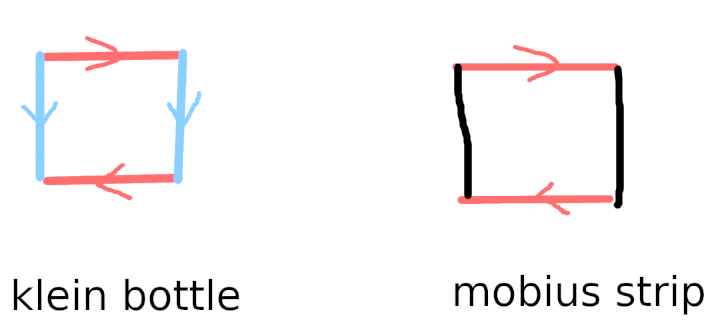
\includegraphics[width=12cm]{fundamental polygons.png}
        \item see diagram
        
        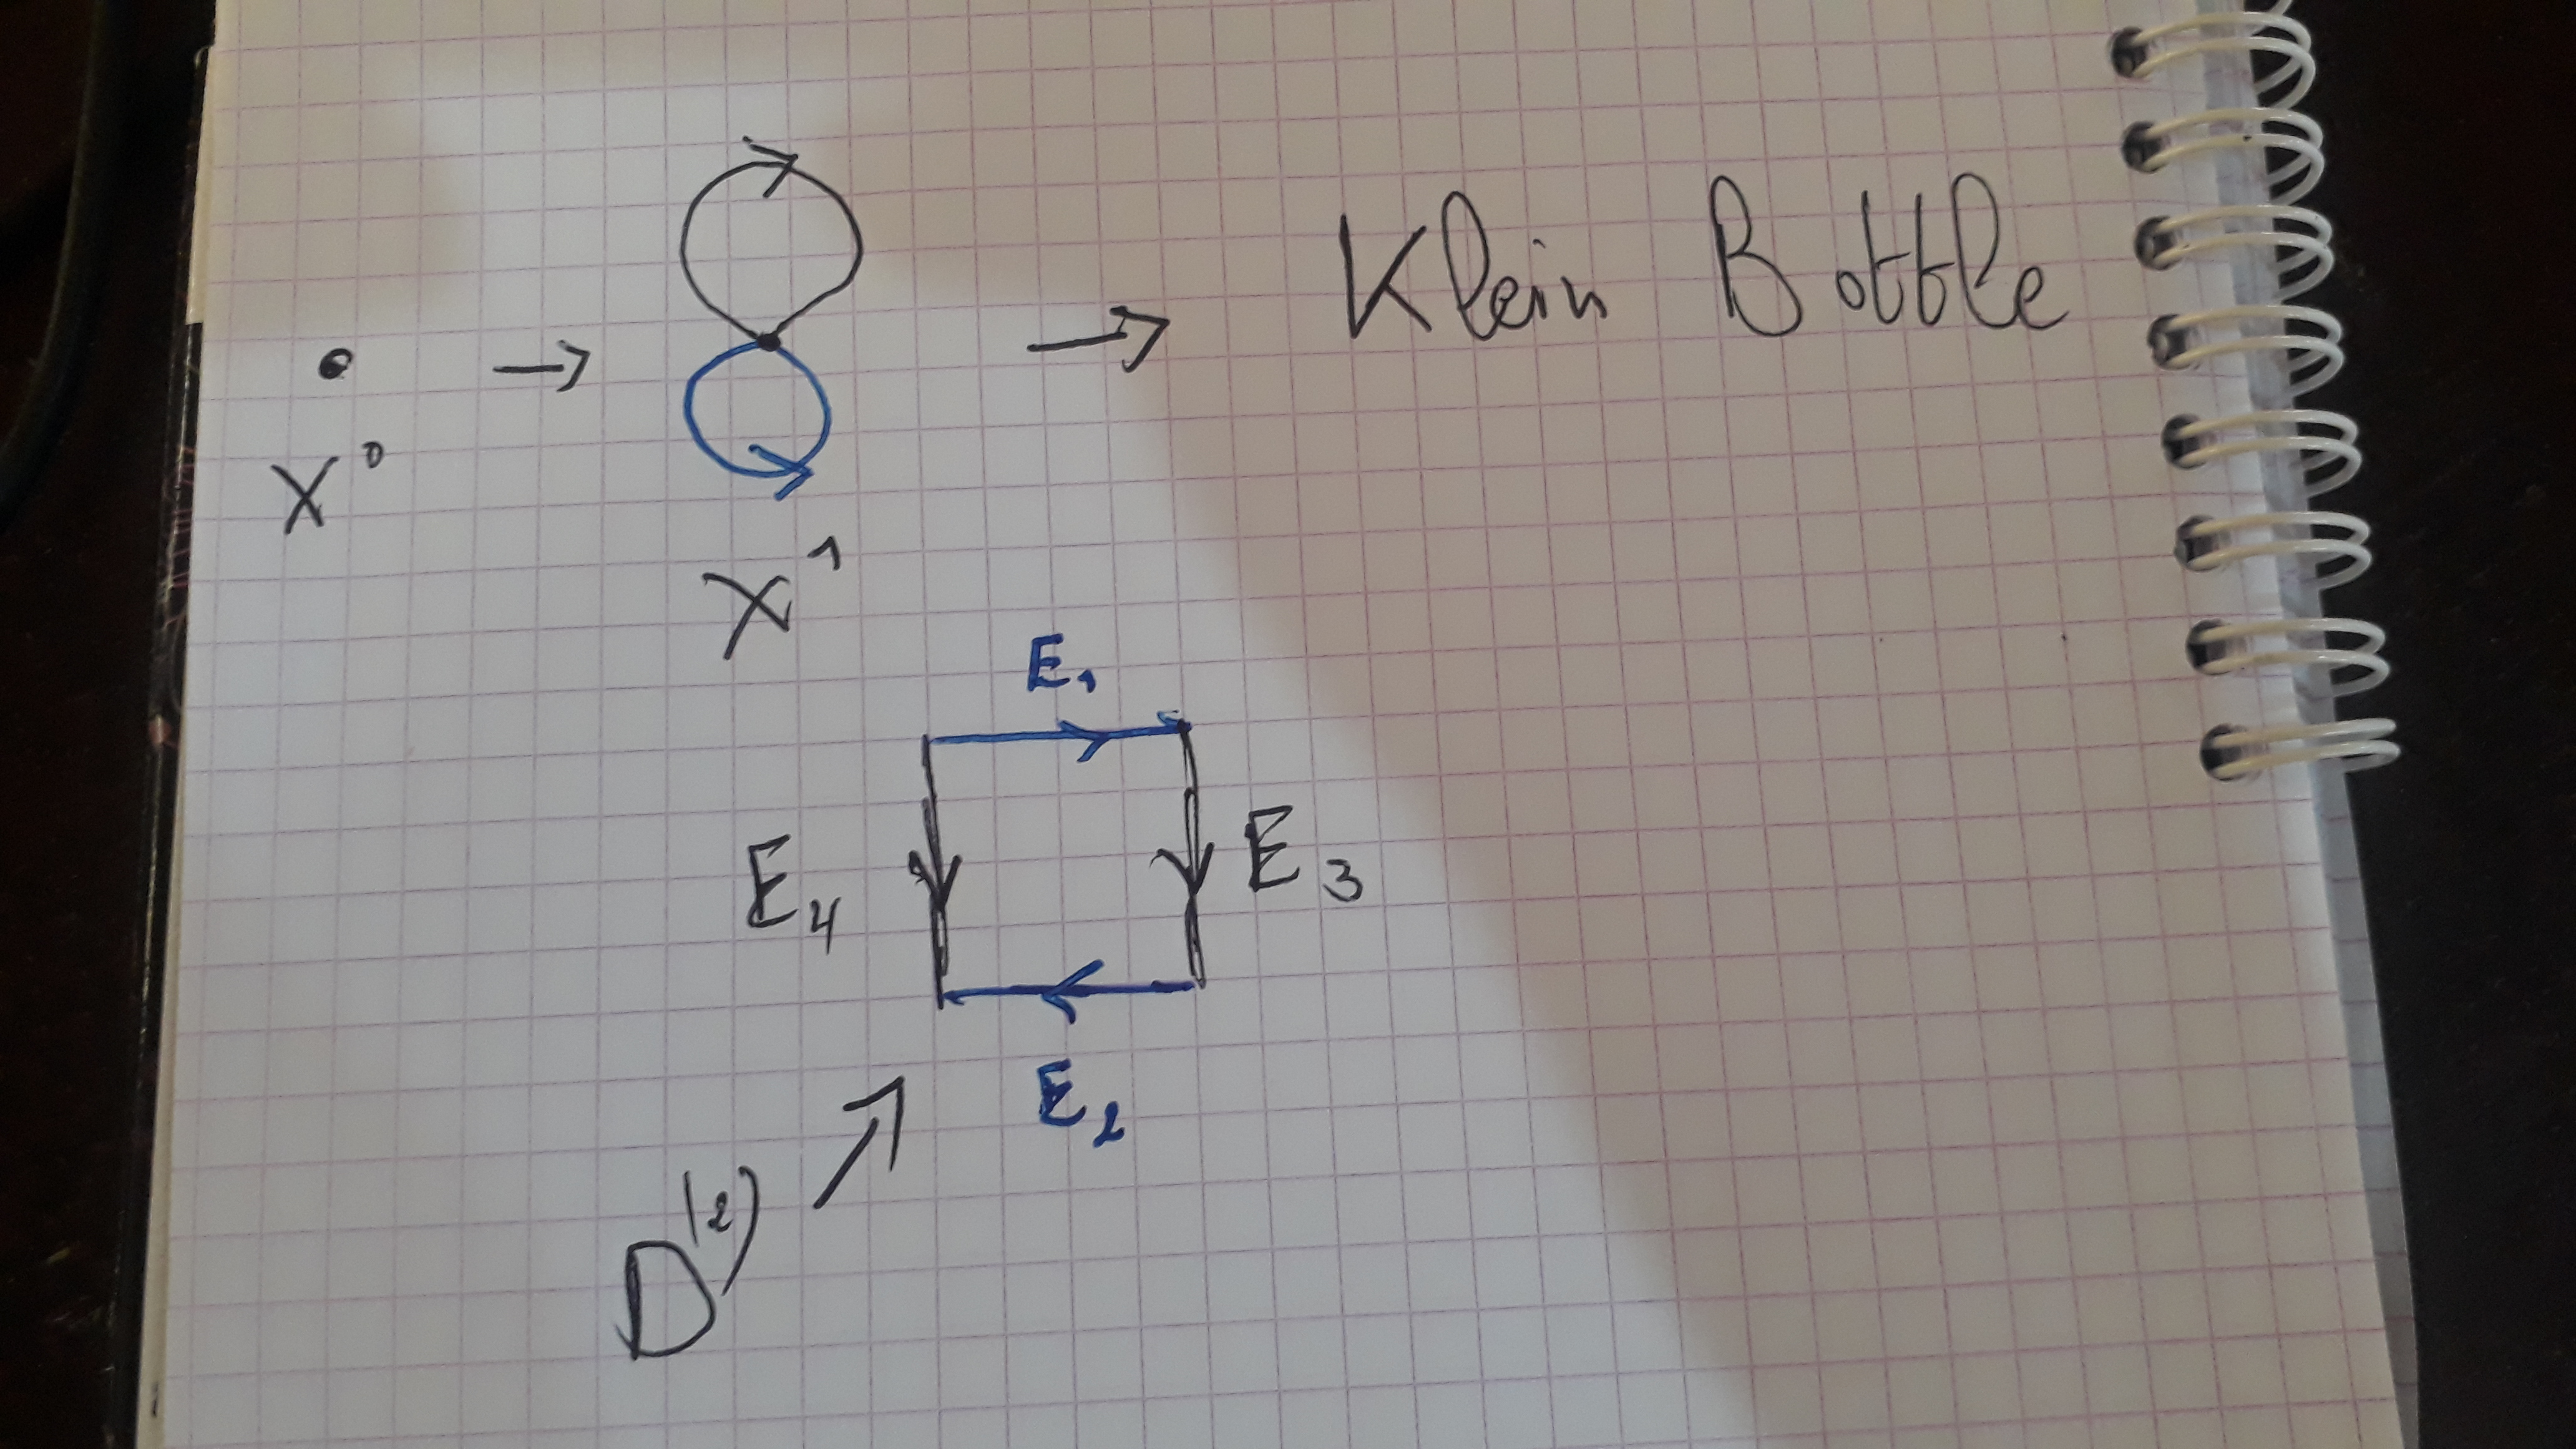
\includegraphics[width=12cm]{cell complex.jpg}
        
        what the attachement map in the last step does is map $E_1$ and $E_2$ to the blue loop in $X^1$ such that the arrows match and the same as well for $E_3$ and $E_4$ onto the black loop. This is a continuous map since the restriction to each edge is continuous and the restrictions agree at the edges. Hence we get a continuous map $\partial D^{(2)}\xlongrightarrow{\varphi} X^1$.
        \item it's apparent from the fundamental polygons that attaching two mobius strips along their boundary circle is equivalent to identifying the two black edges together which coincides with what the fundamental polygon of the klein bottle tells us to do.
    \end{enumerate}
\end{homeworkProblem}
\begin{homeworkProblem}
    \begin{enumerate}
        \item literally just
        \[f_t(x)=\frac{tx}{\norm{x}}+(1-t)x\]
        lmao
        
        \item let $F\colon X\times I\to X$ be the associated map of the deformation retraction, then $F^{-1}(U)$ is open and it contains ${x}\times I$ which is compact. For all $y \in {x}\times I$ we can find a set $V_y \times (a_y, b_y)$ such that $V_y$ is open in $X$ (since sets of this form make up a basis of the product topology). Hence, the set
        \[\{V_y \times (a_y, b_y) | y \in {x}\times I\}\]
        makes up an open cover of ${x}\times I$ from which we can extract a finite subcover 
        \[\{V_{y_i} \times (a_{y_i}, b_{y_i}) | y_i \in {x}\times I, i\leq N\}\]
        now we can just take the open set $V$ defined as
        \[V = \bigcap_{i=0}^N V_{y_i}\]
        and the restriction of $F$ to $V$ gives the desired homotopy. 

        \item first we notice that
        \begin{align*}
            hfg &= h(fg) \simeq h\mbbm{1} \simeq h \\
            hfg &= (hf)g \simeq \mbbm{1}g \simeq g
        \end{align*}
        hence $h$ and $g$ are homotopic. Hence,
        \[gf \simeq hf \simeq \mbbm{1}\]
        which means $f$ is a homotopy equivalence.

        Now assuming $fg$ and $hf$ are homotopy equivalences then there exists maps $k, k'$ such that $fgk\simeq\mbbm{1}$ and $k'hf\simeq\mbbm{1}$. Thereafter, we can just replace $g$ with $gk$ and $h$ with $k'h$ and the result follows.
        
        \item Let $P(X)$ and $P(Y)$ be the set of path components of $X$ and $Y$ respectively and let $p_X\colon X\to P(X)$ be the map that takes each point in $X$ to the path component it resides in, $p_Y$ is definied similarly. now define $\Theta\colon P(X)\to P(Y)$ such that for all $x\in X$
        \[\Theta(p_X(x))=p_Y(f(x))\]
        This map is well defined since if $x,y\in X$ and there exists a path $\gamma\colon I\to X$ connecting them then $f(x)$ and $f(y)$ reside in the same path component as well since $I\xrightarrow{f\gamma} Y$ connects them. Similarly define $\Omega\colon P(Y)\to P(X)$ as
        \[\Omega(p_Y(y))=p_X(g(y))\]
        hence
        \[\Omega(\Theta(p_X(x)))= \Omega(p_Y(g(x))) = p_X(g(f(x)))\]
        but $fg(x)$ resides in the same path-component as $x$ since the homotopy between $gf$ and $\mbbm{1}$ gives us a path between them. Similar reasoning shows that $\Omega$ is also a right inverse of $\Theta$. Therefore, since $\Theta$ has an inverse, it is a bijection.
    \end{enumerate}
\end{homeworkProblem}

\end{document}
